% Drawing 33/09-2 -- folder 33, batch 09, archive page 175 (PDF page 176).
% Transcription: un triangle rectangle, l'hypoténuse redoublée.
% Kind: right triangle. Method 2 (schematic redraw from the facsimile). Status: ok.
% Notes: Right triangle, right angle at the top right; the hypotenuse is drawn twice.
% Coordinates: 1 unit = 1 mm = 1/100 of the crop width (bbox in page fractions: [0.25, 0.33, 0.43, 0.42]).
% Redrawn by Claude (claude-opus-5-5), issue #73, 2026-11-07; not checked by a human; not compiled (no TeX in the session).
% Rights: reproduces part of the work -- behind RENDER_TRANSCRIPTS, never published by itself.
\documentclass[tikz,border=3pt]{standalone}
\usepackage{amsmath,amssymb}
\usetikzlibrary{patterns,arrows.meta}
\tikzset{pencil/.style={black!45}, struck/.style={black!35}, mark/.style={circle,draw,inner sep=1.3pt}, pt/.style={circle,fill,inner sep=0.9pt}, opt/.style={circle,draw,fill=white,inner sep=1.1pt}}
\begin{document}
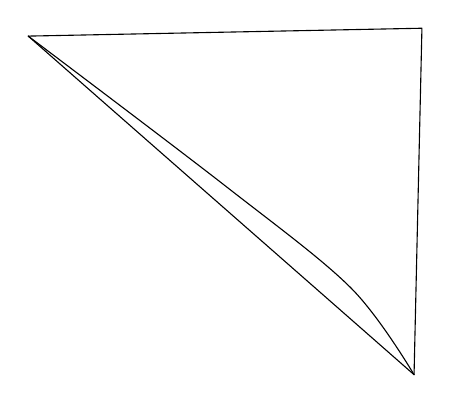
\begin{tikzpicture}[x=1mm,y=1mm,line cap=round,line join=round,font=\scriptsize]
\draw (20,-15) -- (70,-14) -- (69,-58);
\draw (20,-15) -- (69,-58);
\draw plot[smooth, tension=0.55] coordinates {(20,-15) (45,-34) (61,-47) (69,-58)};
\end{tikzpicture}
\end{document}
